\documentclass[12pt,a4paper]{article}
\usepackage[utf8]{inputenc}
\usepackage{amsmath,enumitem,amsfonts,amssymb,graphicx,commath}
\usepackage[width=18.00cm, height=25.00cm]{geometry}
\usepackage{sectsty}
\graphicspath{ {./img/} }

\sectionfont
{\fontsize{14.4}{12}\selectfont}
\title{\textbf{Principles of AI Planning
		\\{\Large Exercise Sheet 7}}}
\makeatletter
\renewcommand{\@maketitle}
{
	\newpage
	\null
	\vskip 2em%
	\begin{center}%
		{\LARGE \@title \\ \par}%
	\end{center}%
	\par
} \makeatother

\begin{document}
\begin{flushleft}
	Authors:\\
	Erick Rosete Beas | er165@uni-freiburg.de\\
	Jessica Lizeth Borja Diaz | jb986@uni-freiburg.de\\
\end{flushleft}
{\let\newpage\relax\maketitle}
\begin{center} 
	\large 13.12.2019 
\end{center}

\section*{Exercise 7.1 - Innacuracy of $h_{max}$}
\textbf{Prove that the heuristic $h_{max}$ is arbitrarily innacurate.}\\
We need to prove that $c \cdot h_{max}(I) \leq h^+(I) \quad \forall c \in R^+$ \\
Select an arbitrary $c$ then we will construct a relaxed planning task $\Pi$ 
where the previous equation holds.\\
The planning task is constructed as follows:\\\\
Given a constant $c$, we select an 
$n$ such that $n \geq c$ where $n$ is a natural number.
\[\Pi = \langle A, I, O^+, \gamma \rangle \]
\[A = \{a_i \mid 1 \leq i \leq n \} \cup \{b_i \mid 1 \leq i \leq n \} \]
\[I = \{ a_i \mapsto 1 \mid 1 \leq i \leq n \} \cup
	  \{ b_i \mapsto 0 \mid 1 \leq i \leq n \} \]
\[O^+ = \{ \langle a_i, b_i \rangle \mid 1 \leq i \leq n  \}\]
\[\gamma = \bigwedge\limits_{i=1}^n b_i \]
By solving this relaxed planning task we can see that\\
\[h_{max}(I) = 1\]
Because when we apply the parallel operators we can reach the goal 
state in one step as all $b_i$ are turned true at the same time.\\
Whereas the minimal amount of sequential operators to be applied 
$h^+(I)$ will be equal to the amount of operators:
\[h^+(I)=n\]
Then:
\[ c \cdot h_{max}(I) \leq h^+(I) \]
\[ \iff c \cdot 1 \leq n \]
\[ \iff n \geq c\]

\section*{Exercise 7.2 - Stability of $h_{add}$ }
\textbf{Show that it is important to test for stability when computing $h_{add}$
by giving an example where you get an unnecessairly high overestimation
when not performing this test.}\\
Consider the following relaxed planning task.\\
\[\Pi = \langle A, I, O^+, \gamma \rangle \]
\[A = \{a_0, a_1, a_2, a_3, a_4 \} \]
\[I = \{ a_0 \mapsto 1, a_1 \mapsto 0, a_2 \mapsto 0,
 a_3 \mapsto 0, a_4 \mapsto 0 \}\]
\[O^+ = \{ \langle a_0, a_1 \rangle, \langle a_1, a_2 \rangle ,
\langle a_2, a_3 \rangle, \langle a_3, a_4 \rangle\}\]
\[\gamma = a_1 \land a_2 \land a_3 \lor a_4 \]
Without a stability test we would get a planning graph as:\\
\begin{center}
	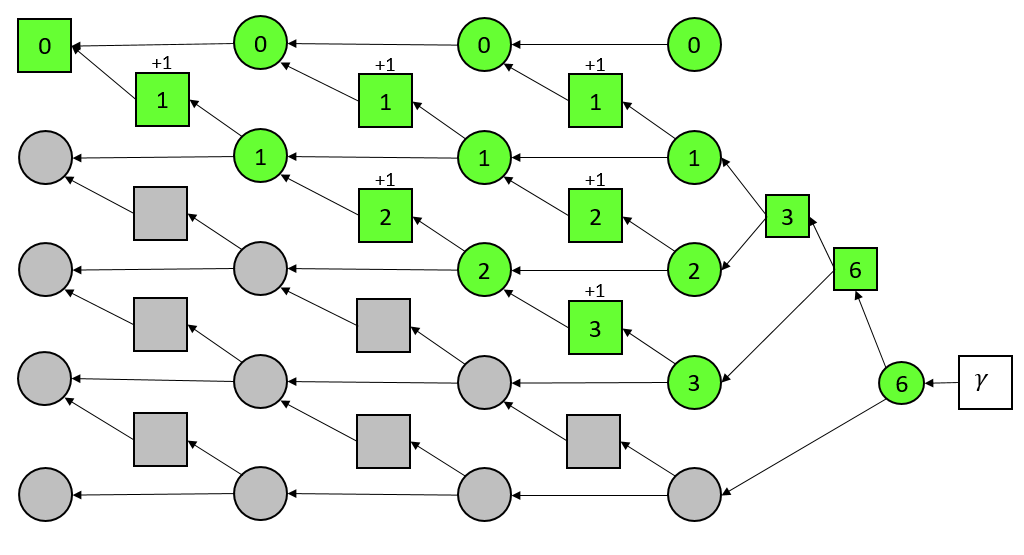
\includegraphics[scale=0.5]{stability_cond.png}\\
\end{center}

With stability test: \\
\begin{center}
	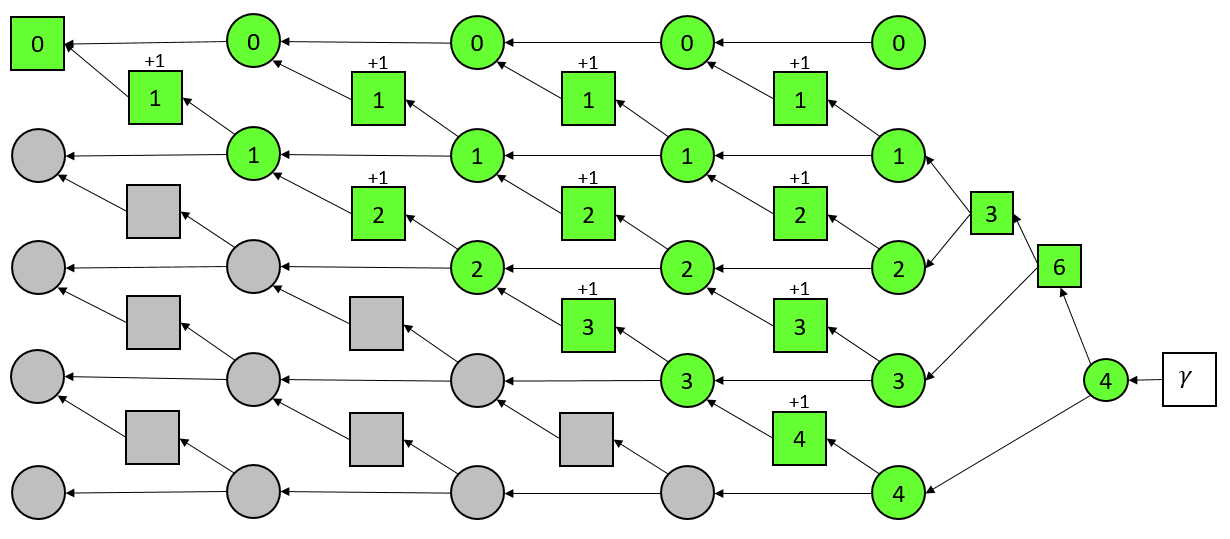
\includegraphics[scale=0.5]{without_stability.png}\\
\end{center}
This means that if we do not wait for the planning graph to be stable
we can overestimate the heuristic when using $h_{add}$.

\newpage
\section*{Exercise 7.3 - Relaxed planning graph and heuristics}

\textbf{Consider the relaxed planning task $\Pi^+$ with variables 
$A=\{a,b,c,d,e\}$, operators $O=\{o_1,o_2,o_3\}$, $o_1=\langle d, c \land (c \triangleright e)\rangle$,
$o_2= \langle c , a \rangle$, $o_3= \langle a, b\rangle$, goal
$\gamma = b \land e$ and initial states $s=\{ a\mapsto 0, 
b\mapsto 0, c \mapsto 0, d \mapsto 1, e \mapsto 0 \}$. Solve the following
by drawing the relaxed planning graph for the lowest depth $k$
that is necessary to extract a solution}
\begin{center}
	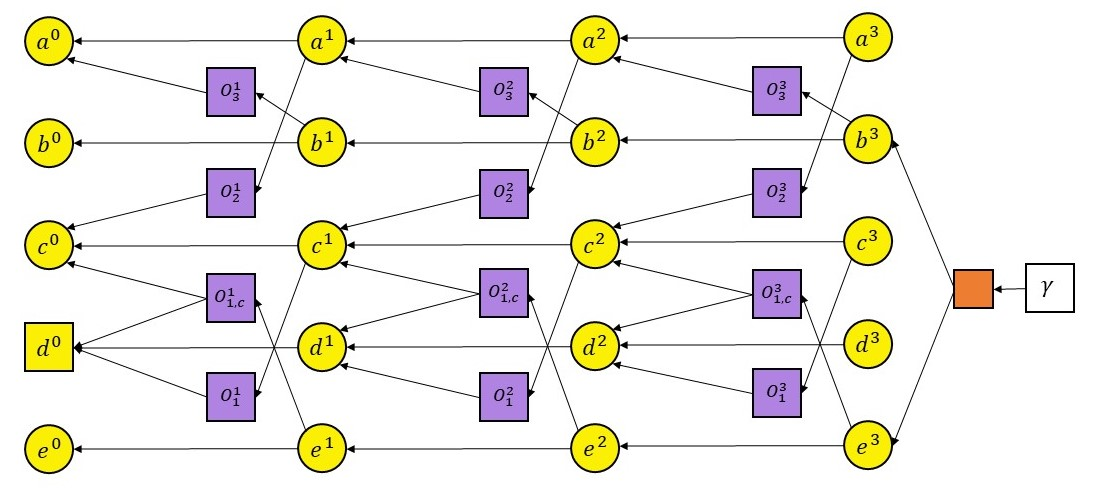
\includegraphics[scale=0.5]{img1.jpg}\\
\end{center}
\begin{enumerate}[label=(\alph*), listparindent=1.5em]
	\item \textbf{Calculate $h_{max}(s)$ for $\Pi^+ $}\\
	\begin{center}
		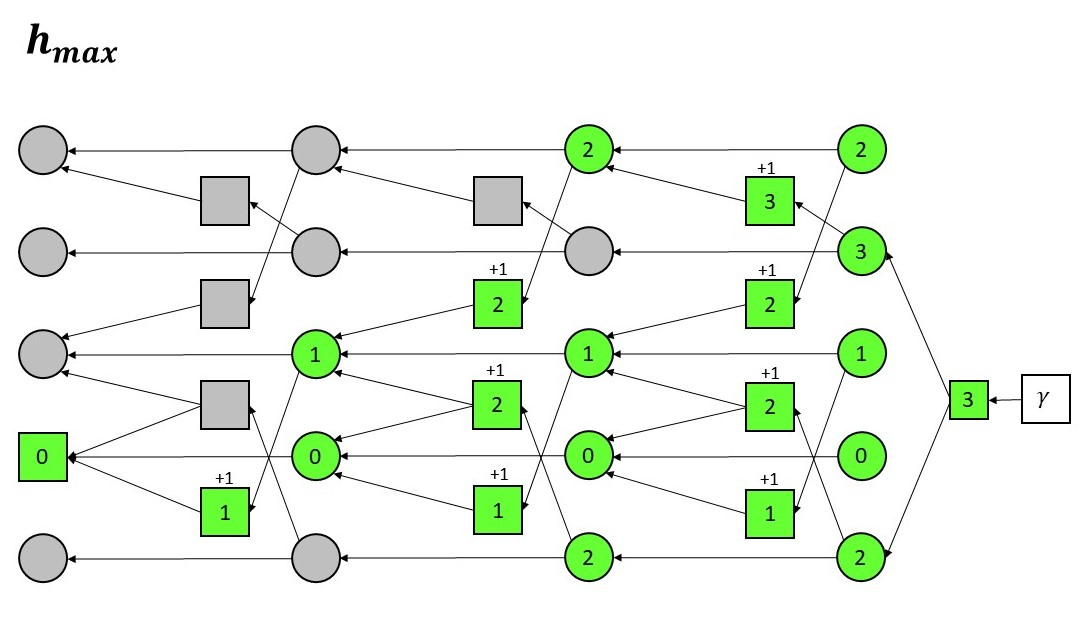
\includegraphics[scale=0.5]{hmax.jpg}\\
	\end{center}
	\newpage
	\item \textbf{Calculate $h_{add}(s)$ for $\Pi^+ $}\\
	\begin{center}
		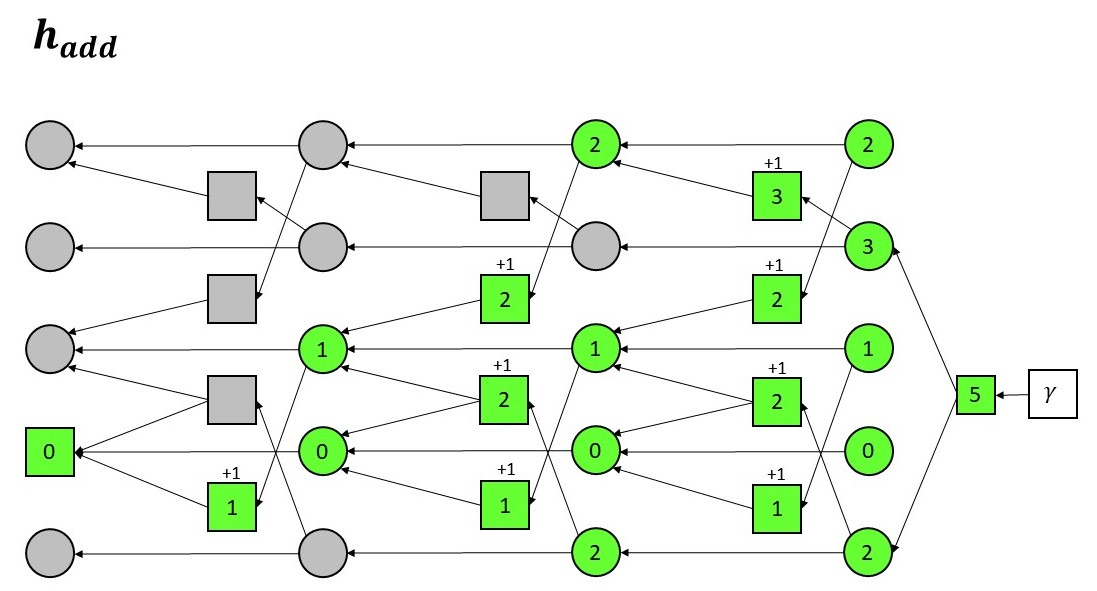
\includegraphics[scale=0.5]{hadd.jpg}\\
	\end{center}

\end{enumerate}
\end{document}